\chapter{Second Order Models}

\section{Modeling Oscillations}
To begin our study of linear second-order differential equations we consider a very simple
physical system: a mass hanging from a spring that is oscillating in time. Figure
\ref{fig:7.8.mass_spring} shows the basic setup for the situation. In Figure
\ref{fig:7.8.mass_spring} the mass is oscillating up and down in the $y$ direction.

\begin{figure}[ht!]
    \begin{center}
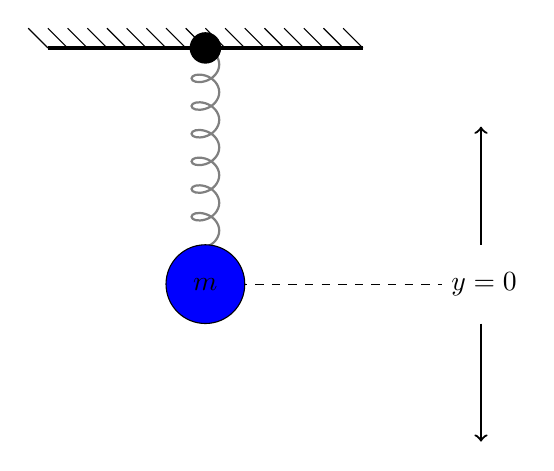
\begin{tikzpicture}
    \draw[ultra thick, black] (-2,0) -- (2,0);
    \foreach \k in {-2,-1.75, -1.5, -1.25, -1, -0.75, -0.5, -0.25,
    0, 0.25, 0.5, 0.75, 1, 1.25, 1.5, 1.75, 2}{
        \draw[black] (\k,0) -- (\k-0.25,0.25);
    }
\draw[thick,gray,decorate,decoration={coil,aspect=0.7,amplitude=5}] (0,0) -- (0,-2.8);
\fill (0,0) circle (.2);
\draw[<-, thick] (3.5,-1) -- (3.5,-2.5);
\draw[->, thick] (3.5,-3.5) -- (3.5,-5);
\draw[dashed, black] (0,-3) -- (3,-3) node[anchor=west]{$y=0$};
\draw[fill=blue] (0,-3) circle(0.5cm) node{$m$};
\end{tikzpicture}
    \end{center}
    \caption{A mass and spring oscillating system.}
    \label{fig:7.8.mass_spring}
\end{figure}

\begin{problem}
    Consider the mass and spring system in Figure \ref{fig:7.8.mass_spring}
    Assuming that the motion is always in the vertical direction, the displacement of the
    mass at time $t$ is $y(t)$, the instantaneous velocity of the mass at the time $t$ is
    $y'(t)$, and the acceleration is $y''(t)$.  Newton's second law: ``mass times
    acceleration equals the sum of the forces'' can be used to write
    \begin{flalign}
        m y''= F_r + F_d + f(t)
        \label{eqn:7.8.mass_spring_basic}
    \end{flalign}
    where $m$ is the mass of the object, $F_r$ is the restoring force due to the spring,
    $F_d$ is the force due to the damping in the system, and $f(t)$ represents any
    external forces on the system.
    \ba
        \item Hooke's Law states that the restoring force of the spring is proportional to
            its displacement.  Use the statement of Hooke's law to propose an expression
            for the restoring force $F_r$.  The constant of proportionality is called the
            {\it spring constant}. Keep in mind that the restoring force works opposite
            the displacement so be sure to get the sign correct.
        \item The damping force $F_d$ is assumed to be proportional to the velocity and
            acts in the direction opposite the direction of motion.  Use this statement to
            propose an expression for the damping force $F_d$. The constant of
            proportionality is called the {\it damping constant}. Keep in mind that the
            damping force works opposite the velocity so be sure to get the sign correct.
        \item If $f(t)$ is any external force acting on the system then we can finally
            write a differential equation describing the motion of the mass and spring
            system.  Write this system and give a full description of each of the
            coefficients.
        \item What are the units of the coefficients given that the units of force are
            Newtons and 
            \[ 1 \text{ Newton} = \frac{1 \text{kg} \cdot \text{m}}{\text{s}^2}. \]
    \ea
\end{problem}



In previous problem we saw a system of the form 
\begin{flalign}
    m y'' = -ky - by' + f(t).
    \label{eqn:7.8.mass_spring1}
\end{flalign}
This equation can be rearranged to 
\begin{flalign}
    m y'' + by'+ky  = f(t).
    \label{eqn:7.8.mass_spring2}
\end{flalign}
The dynamics of this equation are both very interesting and complex.  To get started
consider the next problem.

\begin{problem}
    Go to the GeoGebra applet \\
    \href{http://www.geogebratube.org/student/m217165}{http://www.geogebratube.org/student/m217165}
    \\
    This applet is designed to allow you to explore the mass spring system
    \[ my'' + by' + ky = f(t) \]
    \ba
        \item We will start with an un-driven mass spring system where the forcing
            function is zero. In each of the following cases, sketch a plot of the typical
            behavior seen.
            \begin{enumerate}
                \item Pick several $m$, $b$, and $k$ values that generate an over damped
                    system. An over damped system has the feature that $b^2-4mk>0$.  What
                    physical situation would this scenario model?
                \item Pick several $m$, $b$, and $k$ values that generate a critically
                    damped system. A critically damped system has the feature that
                    $b^2-4mk=0$.  What
                    physical situation would this scenario model?
                \item Pick several $m$, $b$, and $k$ values that generate an under damped
                    system. An under damped system has the feature that $b^2-4mk<0$.  What
                    physical situation would this scenario model?
            \end{enumerate}

        \item Now experiment with a forced spring mass system.  Get a feel for what
            different forcing terms do to control the behavior of the system.

    \ea
\end{problem}


\section{Homogeneous Linear $2^{nd}$ Order Differential Equations}
To begin our study of linear second order equations we need to first examine the
homogeneous equation
\begin{flalign}
    my'' + by' + ky = 0
    \label{eqn:7.8.second_order_hom}
\end{flalign}
where $m,b,k$ are real numbers and $m \ne 0$.  Taking a clue from the method of
undetermined coefficients we can guess the type of solution to be some sort of
exponential function: 
\[ \text{Guess: } y(t) = e^{rt}. \]
Under this guess we can observe that $y'(t) = re^{rt}$ and $y''(t) = r^2 e^{rt}$ to 
rewrite equation \eqref{eqn:7.8.second_order_hom} as
\[ m r^2 e^{rt} + b r e^{rt} + k e^{rt} = 0. \]
After some algebra we see that 
\begin{flalign}
    e^{rt} \cdot \left( mr^2 + br + k \right) = 0. 
    \label{eqn:7.8.charpoly1}
\end{flalign}

The exponential function is never zero when $r$ is a real number so equation
\eqref{eqn:7.8.charpoly1} only has a solution if $mr^2 + br + k = 0$. The left-hand side
of this equation is called the {\it characteristic polynomial} of the differential
equation.
\begin{definition}
    If $my'' + by' + ky = 0$ then the {\it characteristic polynomial} associated with the
    differential equation is
    \begin{flalign}
        p(r) = mr^2 + br + k.
        \label{eqn:7.8.char_poly}
    \end{flalign}
\end{definition}

Since equation \eqref{eqn:7.8.char_poly} is a quadratic equation the solutions can be
found via the quadratic formula
\[ r = \frac{-b \pm \sqrt{b^2 - 4mk}}{2m}. \]
There are typically two solutions, $r_1$ and $r_2$, to the quadratic equation (or two
repeated roots), and using the guess that $y(t) = e^{rt}$ we can write the solutions to
\eqref{eqn:7.8.second_order_hom} as
\[ y(t) = C_1 e^{r_1 t} + C_2 e^{r_2 t}. \]
Recall from high school algebra that it is is possible that there are imaginary solutions
or repeated solutions to a quadratic equation like $p(r)$.  In these cases we take a
slightly different form of the solution.
To classify the solutions to the differential equation \eqref{eqn:7.8.second_order_hom}
recall that the {\bf discriminant} of the quadratic function is $D = b^2 - 4mk$, and this
corresponds to the possibilities listed in the following theorem.

\begin{thm}
    If $my'' + by' + ky = 0$ then a typical solution takes the form $y(t) = e^{rt}$ and the
    characteristic polynomial is $p(r) = mr^2 + br + k$. There are three cases for the
    solutions that each depend on the discriminant $D=b^2 - 4mk$ of the characteristic
    polynomial. 
\begin{center}
    \begin{tabular}{|c|c|c|}
        \hline
        Discriminant: $b^2 - 4mk$ & Roots of $p(r)$ & General Solution\\ \hline \hline
        %
        $b^2 - 4mk > 0$ & 2 Roots: $r_1 \ne r_2$ & $y(t) = C_1 e^{r_1t} + C_2
        e^{r_2t}$  \\ \hline
        %
        $b^2-4mk=0$ & Single root: $r$ & $y(t) = C_1 e^{rt} + C_2 t e^{rt}$ \\ \hline
        %
        $b^2-4mk<0$ & Complex roots: $\alpha \pm \beta i$ & $y(t) = C_1 e^{\alpha t}
        \cos(\beta t) + C_2 e^{\alpha t} \sin(\beta t)$  \\ \hline
    \end{tabular}
\end{center}
\label{thm:7.8.second_hom_soln}
\end{thm}

In each case of Theorem \ref{thm:7.8.second_hom_soln} we see that there are two unknown
constants.  In order to find both constants there need to be 2 conditions: an initial
displacement $y(0)$ and an initial velocity $y'(0)$.
The following examples show the typical solutions of various homogeneous linear second
order differential equations. 



\begin{example}\label{ex:7.8.ex1}
Consider the second order linear homogeneous differential equation $y'' + 4y' + 3y = 0$.
Find the general solution to this differential equation.
\\{\bf Solution:}
If we tie this example to the mass and spring system we have a mass of $m=1$kg, a damping
force of $b=4$kg/s, and a spring constant of $k=3$N/m.  The damping force is {\it rather
high} in comparison to the restoring force so it is expected that the spring mass system
will lose oscillations rather quickly.

The discriminant is $D = b^2 - 4ac = 16-4(1)(3)=4$ so the two roots of the characteristic
polynomial are
\[ r_1 = \frac{-4 + \sqrt{4}}{2} = -1 \quad \text{and} \quad r_2 = \frac{-4 - \sqrt{4}}{2}
    = -3 \]
and by Theorem \ref{thm:7.8.second_hom_soln} we see that the general solution to $y'' +
4y'+3y=0$ is
\[ y(t) = C_1 e^{-1t} + C_2 e^{-3t} \]
This is an infinite collection of possible solutions that depend on two constants
$C_1$ and $C_2$.  In order to have a single solution we must specify an initial
condition $y(0)$ and an initial velocity $y'(0)$.

Figure \ref{fig:7.8.ex2} shows several solutions to the differential equation $y'' +
4y'+3y=0$ with various initial displacements and initial velocities. With a
damping force of $b=4$kg/s this ``mass and spring system'' is working in an
environment where the motion is damped rather quickly.  Imagine that we are
running the experiment in honey!
\end{example}

\begin{figure}[ht!]
    \begin{center}
        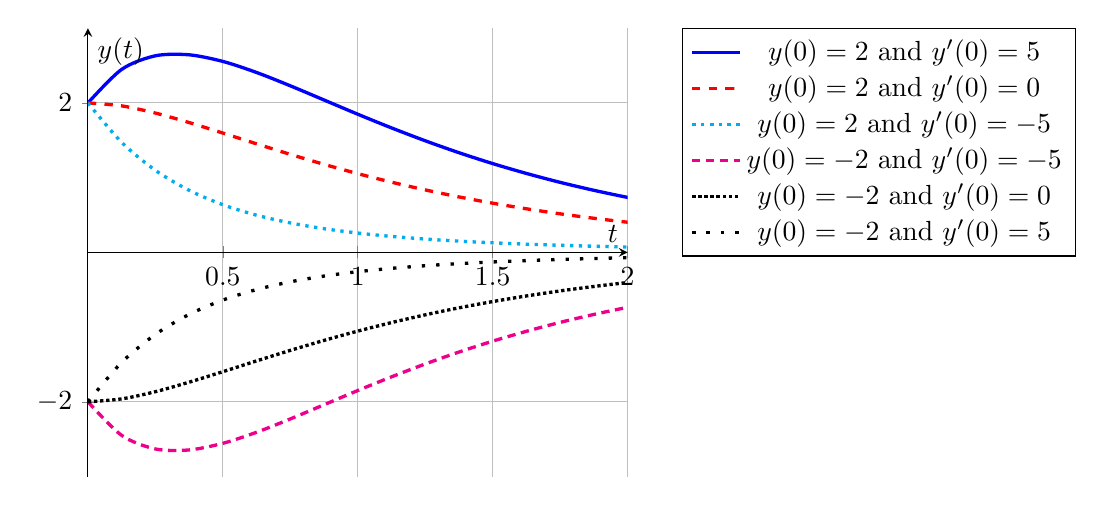
\begin{tikzpicture}
            \begin{axis}[axis lines=center, grid, xmin=0, xmax=2, ymin=-3, ymax=3, grid,
                legend style={at={( 1.1,1)}, anchor=north west}, xlabel={$t$},
            ylabel={$y(t)$}]
                \addplot[smooth, very thick, blue, domain=0:3] {5.5*exp(-1*x)-3.5*exp(-3*x)};
                \addlegendentry{$y(0) = 2$ and $y'(0) = 5$};
                \addplot[smooth, very thick, red, dashed, domain=0:3] {3*exp(-1*x)-1*exp(-3*x)};
                \addlegendentry{$y(0) = 2$ and $y'(0) = 0$};
                \addplot[smooth, very thick, cyan, dotted, domain=0:3] {0.5*exp(-1*x)+1.5*exp(-3*x)};
                \addlegendentry{$y(0) = 2$ and $y'(0) = -5$};
                \addplot[smooth, very thick, magenta, densely dashed, domain=0:3]
                {-5.5*exp(-1*x)+3.5*exp(-3*x)};
                \addlegendentry{$y(0) = -2$ and $y'(0) = -5$};
                \addplot[smooth, very thick, black, densely dotted, domain=0:3]
                {-3*exp(-1*x)+1*exp(-3*x)};
                \addlegendentry{$y(0) = -2$ and $y'(0) = 0$};
                \addplot[smooth, very thick, black, loosely dotted, domain=0:3]
                {-0.5*exp(-1*x)-1.5*exp(-3*x)};
                \addlegendentry{$y(0) = -2$ and $y'(0) = 5$};
            \end{axis}
        \end{tikzpicture}
    \end{center}
    \caption{Several solutions to $y''+4y'+3y=0$ shown in example \ref{ex:7.8.ex2}.}
    \label{fig:7.8.ex1}
\end{figure}

\begin{example}\label{ex:7.8.ex2}
Consider the second order linear homogeneous differential equation $y'' + 1y' + 1y = 0$.
Find the general solution to this differential equation.
\\{\bf Solution:}
If we tie this example to the mass and spring system we have a mass of $m=1$kg, a damping
force of $b=1$kg/s, and a spring constant of $k=1$N/m.  In this case the spring constant
(the restoring force) and the damping force will play against each other to create a
damped oscillator.

The discriminant is $D = b^2-4ac = 1-4(1)(1)=-3$.  Since the discriminant is negative we
will have the sine and cosine solution on the third line of the table in Theorem
\ref{thm:7.8.second_hom_soln}.
\[ r_1 = \frac{-1 + \sqrt{-3}}{2} = -\frac{1}{2} + \frac{\sqrt{3}}{2} i \quad \text{and}
    \quad r_2 = \frac{-1-\sqrt{-3}}{2} = -\frac{1}{2} - \frac{\sqrt{3}}{2} i.\]
    If we define $\alpha = -1/2$ and $\beta = -\frac{\sqrt{3}}{2}$ we get the general solution to $y''+y+1=0$
as
\[ y(t) = C_1 e^{\alpha t} \cos(\beta t) + C_2 e^{\alpha t} \sin(\beta t) \]
\[\implies  y(t) = C_1 e^{-1/2 t} \cos\left( \frac{\sqrt{3}}{2} t \right) + C_2 e^{-1/2 t} \sin
    \left( \frac{\sqrt{3}}{2} t \right). \]
Since there are two constants this is an infinite collection of solutions that depend on
the initial displacement $y(0)$ and the initial velocity $y'(0)$. Figure \ref{fig:7.8.ex2}
shows several solutions.

\end{example}


\begin{figure}[ht!]
    \begin{center}
        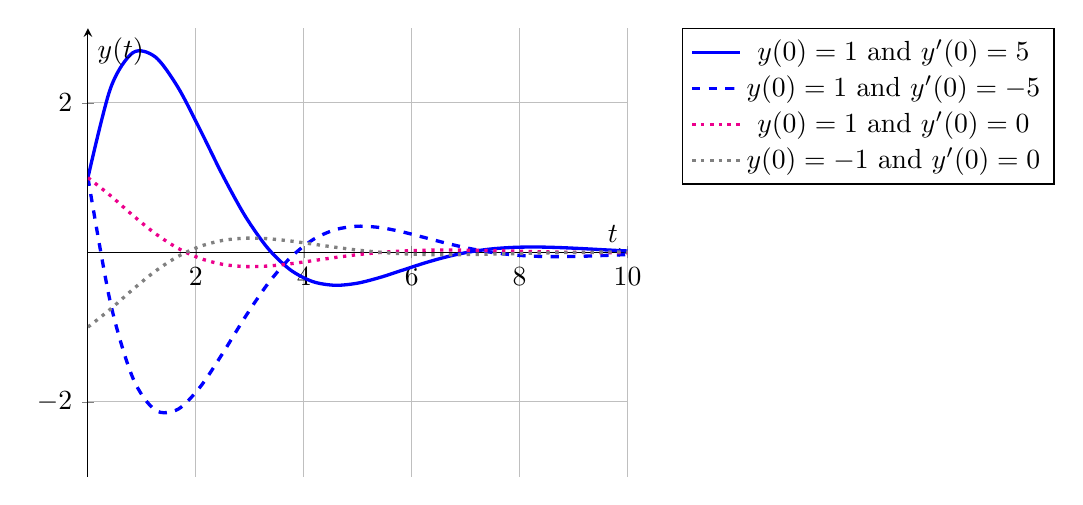
\begin{tikzpicture}
            \begin{axis}[axis lines=center, grid, xmin=0, xmax=10, ymin=-3, ymax=3, grid,
                legend style={at={( 1.1,1)}, anchor=north west}, xlabel={$t$},
            ylabel={$y(t)$}]
                \addplot[smooth, very thick, blue, domain=0:10]
                {1*exp(-0.5*x)*cos(0.866*deg(x))+5*exp(-0.5*x)*sin(0.866*deg(x))};
                \addlegendentry{$y(0) = 1$ and $y'(0) = 5$};
                \addplot[smooth, very thick, blue, dashed, domain=0:10]
                {1*exp(-0.5*x)*cos(0.866*deg(x))-5*exp(-0.5*x)*sin(0.866*deg(x))};
                \addlegendentry{$y(0) = 1$ and $y'(0) = -5$};
                \addplot[smooth, very thick, magenta, dotted, domain=0:10]
                {1*exp(-0.5*x)*cos(0.866*deg(x))+0*exp(-0.5*x)*sin(0.866*deg(x))};
                \addlegendentry{$y(0) = 1$ and $y'(0) = 0$};
                \addplot[smooth, very thick, gray, dotted, domain=0:10]
                {-1*exp(-0.5*x)*cos(0.866*deg(x))+0*exp(-0.5*x)*sin(0.866*deg(x))};
                \addlegendentry{$y(0) = -1$ and $y'(0) = 0$};
            \end{axis}
        \end{tikzpicture}
    \end{center}
    \caption{Several solutions to $y''+y'+y=0$ shown in example \ref{ex:7.8.ex2}. Notice
that this equation models an underdamped oscillator where some oscillations occur.}
    \label{fig:7.8.ex2}
\end{figure}



\begin{example}\label{ex:7.8.ex3}
Consider the second order linear homogeneous differential equation $y''+6y'+9y=0$. Find
the general solution to this differential equation.
\\{\bf Solution:}
The discriminant is $D=b^2-4ac = 6^2-4(1)(9)=36-36=0$.  This is the second case in the
table in Theorem \ref{thm:7.8.second_hom_soln}; a repeated root
\[ r = \frac{-6 \pm \sqrt{0}}{2} = -3. \]
The solution is therefore
\[ y(t) = C_1 e^{-3t} + C_2 t e^{-3t}. \]
As in the previous two examples there are infinitely many solutions that depend on the
initial condition $y(0)$ and initial velocity $y'(0)$. Figure \ref{fig:7.8.ex3} shows
several solutions.
\end{example}

\begin{figure}[ht!]
    \begin{center}
        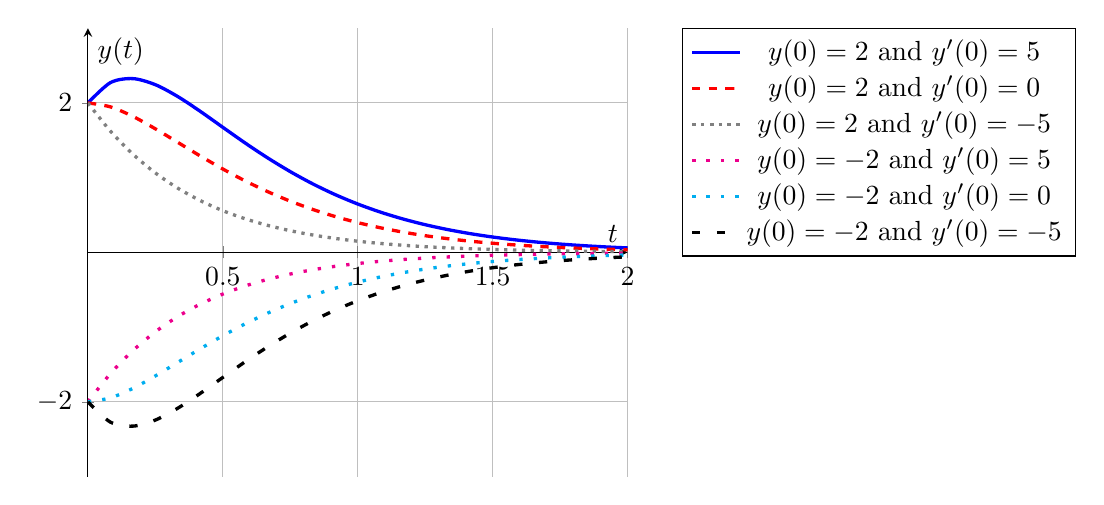
\begin{tikzpicture}
            \begin{axis}[axis lines=center, grid, xmin=0, xmax=2, ymin=-3, ymax=3, grid,
                legend style={at={( 1.1,1)}, anchor=north west}, xlabel={$t$},
            ylabel={$y(t)$}]
                \addplot[smooth, very thick, blue, domain=0:2] {2*exp(-3*x)+11*x*exp(-3*x)};
                \addlegendentry{$y(0) = 2$ and $y'(0) = 5$};
                \addplot[smooth, very thick, red, dashed, domain=0:2] {2*exp(-3*x)+6*x*exp(-3*x)};
                \addlegendentry{$y(0) = 2$ and $y'(0) = 0$};
                \addplot[smooth, very thick, gray, dotted, domain=0:2] {2*exp(-3*x)+1*x*exp(-3*x)};
                \addlegendentry{$y(0) = 2$ and $y'(0) = -5$};
                \addplot[smooth, very thick, magenta, loosely dotted, domain=0:2] {-2*exp(-3*x)-1*x*exp(-3*x)};
                \addlegendentry{$y(0) = -2$ and $y'(0) = 5$};
                \addplot[smooth, very thick, cyan, loosely dotted, domain=0:2]
                {-2*exp(-3*x)-6*x*exp(-3*x)};
                \addlegendentry{$y(0) = -2$ and $y'(0) = 0$};
                \addplot[smooth, very thick, black, loosely dashed, domain=0:2] {-2*exp(-3*x)-11*x*exp(-3*x)};
                \addlegendentry{$y(0) = -2$ and $y'(0) = -5$};
            \end{axis}
        \end{tikzpicture}
    \end{center}
    \caption{Several solutions to $y''+6y'+9y=0$ shown in example \ref{ex:7.8.ex3}. This
is a model for a critically damped oscillator where no oscillations can occur..}
    \label{fig:7.8.ex3}
\end{figure}


The mass spring system can be written as $my'' + by' +
ky = 0$ when there is no external forcing.  This has the same form as the second order
linear homogeneous differential equation in Theorem \ref{thm:7.8.second_hom_soln}.  In the
mass spring system, the discriminant is 
\[ D = b^2 - 4(m)(k) \]
and we can classify all such systems with the following definitions.
\begin{definition}
\begin{itemize}
    \item $D = b^2-4mk >0$ \quad The system is {\it over damped}
    \item $D = b^2-4mk =0$ \quad The system is {\it critically damped}
    \item $D = b^2-4mk <0$ \quad The system is {\it under damped}
\end{itemize}
\end{definition}

\begin{thm}
    For the homogeneous mass spring oscillator equation 
    \[ my'' + by' + ky = 0 \]
    with $m, k, b > 0$ there are four primary solution types.
    \begin{description}
        \item[Un-Damped ($b = 0$):]
                \[ y(t) = C_1 \cos(\omega t) + C_2 \sin(\omega t) \]
                where $\omega = \sqrt{\frac{k}{m}}$ is called the natural frequency of the
                oscillator.
        \item[Under Damped (two complex roots):] 
            \[ y(t) = e^{\alpha t} \left( C_1 \cos(\omega t) + C_2
                \sin(\omega t) \right) \]
            where $r = \alpha \pm i \omega$
        \item[Over Damped (two real roots):] 
            \[y(t) = C_1 e^{r_1 t} + C_2 e^{r_2 t}\]
        \item[Critically Damped (one repeated real root):] 
            \[ y(t) = C_1 e^{rt} + C_2 t e^{rt} \]
    \end{description}
\end{thm}




\begin{problem}
Use the equation derived in this chapter to change the descriptions of
the mass spring systems to a second order linear homogeneous differential equation.  Then
solve the equation with the aid of Theorem \ref{thm:7.8.second_hom_soln} and the given
descriptions of the initial displacement and initial velocity. State whether each
situation is an over- or under-damped oscillator.
\ba
    \item An object with a mass of $m=1$kg is suspended from a spring with a spring
        constant $k=4$N/m.  The system is submerged in a liquid causing it to have a large
        damping constant $b=5$kg/s. The object is lifted up $1$meter and let go with no
        initial velocity.
    \item An object with a mass of $m=1$kg is suspended from a spring with a spring
        constant $k=10$N/m.  The system is submerged in a liquid causing it to have a large
        damping constant $b=2$kg/s. The object is pulled down $1$meter and given an
        initial velocity of $1$m/s.
    \item An object with a mass of $m=10$kg is suspended on a spring with spring constant
        $k=20$N/m.  The damping coefficient is $b=30$kg/s. The mass is initially held at
        equilibrium and is given an initial velocity of $2$m/s in the downward direction.
\ea
\end{problem}


\begin{problem}
For each of the following, use the applet
\href{https://www.geogebra.org/m/S4ktuMbX}{https://www.geogebra.org/m/S4ktuMbX} to show
the dynamics of situation before you find the analytic solution.
\begin{enumerate}
    \item Consider a mass-spring system with mass $m=1kg$ and restoring force $k = 4N/m$.
        Let $y(0) = 1$ and $y'(0)=0$.  Find the position function $y(t)$.
        \\\solution{
        The differential equation is: $y'' + 4y = 0$ with $y(0)=1$ and $y'(0) = 0$.
        Assume that $y(t) = e^{rt}$ and observe that the characteristic polynomial is $r^2
        + 4 = 0$ so $r = \pm 2i$.  Therefore the solution is trigonometric and we get
        \[ y(t) = C_1 \sin(2t) + C_2 \cos(2t). \]
        Using the initial condition we get $1 = C_2$ \\
        Taking the derivative of $y$ we get
        \[ y'(t) = 2 C_1 \cos(2t) - 2 C_2 \sin(2t) \]
        and using the initial velocity we get $0 = 2C_1 \implies C_1 = 0$.  Therefore,
        \[ \boxed{y(t) = \cos(2t)} \]
        }
    \item Consider a mass-spring system with mass $m=1kg$ and restoring force $k = 4N/m$.
        Let $y(0) = 0$ and $y'(0)=1$.  Find the position function $y(t)$.
        \\\solution{
        The differential equation is: $y'' + 4y = 0$ with $y(0)=0$ and $y'(0) = 1$.
        Assume that $y(t) = e^{rt}$ and observe that the characteristic polynomial is $r^2
        + 4 = 0$ so $r = \pm 2i$.  Therefore the solution is trigonometric and we get
        \[ y(t) = C_1 \sin(2t) + C_2 \cos(2t). \]
        Using the initial condition we get $0 = C_2$ \\
        Taking the derivative of $y$ we get
        \[ y'(t) = 2 C_1 \cos(2t) - 2 C_2 \sin(2t) \]
        and using the initial velocity we get $1 = 2C_1 \implies C_1 = 0.5$.  Therefore,
        \[ \boxed{y(t) = 0.5\sin(2t)} \]

        }
    \item Consider a mass-spring system with mass $m=9kg$ and restoring force $k = 1N/m$.
        Let $y(0) = 3$ and $y'(0)=0$.  Find the position function $y(t)$.
        \\\solution{
        The differential equation is: $9y'' + y = 0$ with $y(0)=3$ and $y'(0) = 0$.
        Assume that $y(t) = e^{rt}$ and observe that the characteristic polynomial is $9r^2
        + 1 = 0$ so $r = \pm \frac{1}{3}i$.  Therefore the solution is trigonometric and we get
        \[ y(t) = C_1 \sin\left(\frac{1}{3}t\right) + C_2 \cos\left(\frac{1}{3}t\right). \]
        Using the initial condition we get $3 = C_2$ \\
        Taking the derivative of $y$ we get
        \[ y'(t) = \frac{1}{3} C_1 \cos\left( \frac{1}{3} t\right) - \frac{1}{3} C_2
        \sin\left( \frac{1}{3} t\right) \]
        and using the initial velocity we get $0 = \frac{1}{3}C_1 \implies C_1 = 0$.  Therefore,
        \[ \boxed{y(t) = 3\cos\left(\frac{1}{3} t\right) } \]
        }
    \item Consider a mass-spring system with mass $m=2kg$ and restoring force $k = 18N/m$.
        Let $y(0) = 1$ and $y'(0)=-1$.  Find the position function $y(t)$.
        \\\solution{
            The differential equation is: $2y'' + 18y = 0$ with $y(0)=1$ and $y'(0) = -1$.
        Assume that $y(t) = e^{rt}$ and observe that the characteristic polynomial is $2r^2
        + 18 = 0$ so $r = \pm 3i$.  Therefore the solution is trigonometric and we get
        \[ y(t) = C_1 \sin(3t) + C_2 \cos(3t). \]
        Using the initial condition we get $1 = C_2$ \\
        Taking the derivative of $y$ we get
        \[ y'(t) = 3 C_1 \cos(3t) - 3 C_2 \sin(3t) \]
        and using the initial velocity we get $-1 = 3C_1 \implies C_1 =
        -\frac{1}{3}$.  Therefore,
        \[ \boxed{y(t) = -\frac{1}{3}\sin(3t) + \cos(3t)} \]
    }

    \item Consider the motion of a brick with a mass of $m=6kg$ that is hung from the end of
        a spring.  When the brick is at rest, the weight of the brick stretches the spring
        by $0.1 m$, so that the force of gravity down is equal to the force of the spring
        pulling up. 
        \begin{enumerate}
            \item The weight the force of gravity on the brick, is equal to the brick's
                mass multiplied by $g$, the acceleration of gravity. Use $g = 9.8$ meters
                per second squared to calculate what the spring constant $k$ must be. 
                \\\solution{
                We first approach this problem as a balance of forces.  If the weight,
                $mg$, is balanced by the spring constant and the stretch in the spring
                then $(6)(9.8) = k(0.09)$ which means that $k = (6\cdot 9.8)/0.1 =588$
                }
            \item Set up a differential equation for the motion of the brick.
                \\\solution{$y''+588y=0$}
            \item The spring is then stretched 0.11 m away from equilibrium and released.
                To describe the motion, set up a differential equation with initial
                conditions. 
                \\\solution{
                $y(0) = 0.11$ and $y'(0) = 0$.  Also, the characteristic polynomial is
                $r^2 + 588 = 0$ so the roots are $r = \pm \sqrt{588} i$.  This gives a
                general solution of
                \[ y(t) = C_1 \sin(\sqrt{588} t) + C_2 \cos(\sqrt{588} t). \]
                Using the initial condition we have $0.11 = C_2$.  Taking the derivative
                of the function gives
                \[ y'(t) = \sqrt{588} C_1 \cos(\sqrt{588}t) - \sqrt{588} C_2
                \sin(\sqrt{588} t) \]
                Hence, with the initial velocity we see that $C_1 = 0$.  Therefore,
                \[ \boxed{y(t) = 0.11 \cos(\sqrt{588} t) } \]
                }
        \end{enumerate}

\end{enumerate}
\end{problem}


\begin{problem}
Recall that in a spring-mass system Newton's second law gives:
\[ my'' = F_r + F_d \]
where 
\begin{itemize}
    \item $m$ is the mass, 
    \item $F_r$ is the restoring force (which is proportional to the
displacement), and
    \item $F_d$ is the damping force (which is proprotion to the velocity).
\end{itemize}
Hence, the motion is governed by the equation
\[ my'' = -ky - by' \]
and after some algebra we get
\[ my'' + by' + ky = 0 \]
\begin{enumerate}
    \item Consider spring-mass system with mass $m=1kg$, damping force $b=3\, kg/s$, and
        restoring force $k=2\,N/m$.  If $y(0)=1$ and $y'(0)=0$ then find the function
        modeling the position: $y(t)$. 
        \\\solution{
        The equation is $y''+3y'+2y=0$ and guessing that $y(t) = e^{rt}$ gives the
        characteristic polynomial $r^2 + 3r + 2 = 0$.  This polynomial is factorable so we
        have $(r+1)(r+2) = 0$ which yields the roots $r=-1,-2$.  Hence,
        \[ y(t) = C_1 e^{-t} + C_2 e^{-2t}. \]
        Using the initial condition we get $C_1 + C_2 = 1$.  Taking the derivative we get
        \[ y'(t) = -C_1 e^{-t} -2C_2 e^{-2t} \]
        so from the initial velocity we get $0 = -C_1 - 2C_2$.  Therefore we can solve the
        system with matrices:
        \[ \left( \begin{array}{cc|c} 1 & 1 & 1 \\ -1 & -2 & 0 \end{array} \right) \to
            \cdots \to
        \left( \begin{array}{cc|c} 1 & 0 & 2 \\ 0 & 1 & -1 \end{array} \right) \]
        so 
        \[ \boxed{y(t) = 2 e^{-t} - e^{-2t}} \]
        }

    \item Consider spring-mass system with mass $m=1kg$, damping force $b=2\, kg/s$, and
        restoring force $k=1\,N/m$.  If $y(0)=0$ and $y'(0)=1$ then find the function
        modeling the position: $y(t)$. 
        \\\solution{
        The equation is $y''+2y'+1y=0$ and guessing that $y(t) = e^{rt}$ gives the
        characteristic polynomial $r^2 + 2r + 1 = 0$.  This polynomial is factorable so we
        have $(r+1)(r+1) = 0$ which yields the roots $r=-1,-1$.  This is a repeated root
        so our two solutions won't be linearly indepdent.  Hence,
        \[ y(t) = C_1\cdot e^{-t} + C_2 \cdot t \cdot e^{-t}. \]
        Using the initial condition we get $C_1 = 0$.  Taking the derivative (with the
        product rule) we get
        \[ y'(t) = -C_1 e^{-t} + C_2 \left( -t e^{-t} + e^{-t}\right) \]
        so from the initial velocity we get $1 = -C_1 + C_2$. Hence, $C_2 = 1$ and
        \[ \boxed{y(t) = t e^{-t}} \]
        }


    \item Consider spring-mass system with mass $m=2kg$, damping force $b=4\, kg/s$, and
        restoring force $k=4\,N/m$.  If $y(0)=1$ and $y'(0)=0$ then find the function
        modeling the position: $y(t)$. 
        \\\solution{
        The equation is $2y''+4y'+4y=0$ with $y(0) = 1$ and $y'(0) = 0$.  Guessing that
        $y(t) = e^{rt}$ gives the characteristic polynomial $2r^2+4y+4=0$.  Using the
        quadratic formula we get
        \[ r = \frac{-4 \pm \sqrt{16-4(2)(4)}}{2(2)} = \frac{-4 \pm \sqrt{-16}}{4} =
        \frac{-4 \pm 4i}{4} = -1 \pm i \]
        Let $\alpha = -1$ and $\beta = 1$ as we get
        \[ y(t) = e^{-t} \left( C_1 \cos(t) + C_2 \sin(t)\right) \]
        Using the initial condition we see that $1 = C_1$.  Taking the derivative (with
        the product aand chain rules) we get
        \[ y'(t) = e^{-t} \left( -C_1 \sin(t) + C_2 \cos(t) \right) - e^{-t} \left( C_1
        \cos(t) + C_2 \sin(t) \right). \]
        Using the initial velocity we get
        \[ 0 = C_2 - C_1. \]
        Therefore $C_2 = 1$ and 
        \[ y(t) = e^{-t} \left( \cos(t) + \sin(t) \right) \]
        }
\end{enumerate}
\end{problem}


\begin{problem}
    Classify each of the scenarios from the previous two problems as ``undamped'', ``under
    damped'', ``critically damped'', or ``over damped''.
\end{problem}


\section{Forced Oscillations}
In the previous Section we encountered the mass spring system 
\[ my'' + by' + ky = 0 \]
where $m$ is the mass of the object, $b$ is the damping term, and $k$ is the restoring
force called the spring constant.  In the present situation we will consider what happens
with the right-hand side is not zero, but instead if there is an external force acting
driving (or working in opposition to) the oscillations.  The following Preview Activity
will get you started.

% \input{previews/7.9.PA1}
\begin{problem}
    For a nonhomogeneous linear differential equation, the general solution takes the form
    \[ y(t) = y_h(t) + y_p(t) \]
    where $y_h(t)$ is the homogeneous solution and $y_p(t)$ is the particular solution
    given the nonhomogeneity.  For each of the following second
    order linear nonhomogeneous differential equations, write the homogeneous solution
    and a possible particular solution.
    \ba
        \item $y''+5y'+6y=\sin(2t)$
        \item $y''+4y=e^{-t}$
        \item $y''+6y'+9y=2+t$
    \ea
\end{problem}

\subsection*{Resonance}
Consider an undamped mass spring system forced by an oscillating term with amplitude $R$
and a frequency $\omega$.
\[ my''+ ky = R \sin(\omega t). \]
The homogeneous solution can be found by solving $my''+ky=0$ and the particular solution
will take the form of a sinusoidal function with frequency $\omega$.  The {\bf natural
frequency} of the homogeneous equation is $\omega_0 = \sqrt{k/m}$ by Theorem
\ref{thm:7.8.second_hom_soln}.  When the natural frequency of the homogeneous solution and
the natural frequency of the forcing term match we get the phenomenon called {\bf
resonance.}

The following activity will walk you through solving problems with resonance.

% \input{activities/7.9.Act1}
\begin{problem}
    Consider differential equation $y''+4y = \sin(2t)$. This can be viewed as a mass
    spring system with a restoring force of $k=4$, no damping force $b=0$ and a forcing
    term $f(t) = \sin(2t)$.
    \ba
        \item Use the ideas from the previous Section to write a general
            solution to the homogeneous equation $y''+4y=0$.
        \item Conjecture the form of the particular solution $y_p(t)$ that matches the
            form of the nonhomogeneity. In this case the homogeneous solution and the
            particular solution have exactly the same form.  The fix for this is to
            multiply the particular solution by $t$.  Write the particular solution.
        \item Write the solution as the sum of the homogeneous and particular solutions
            $y(t) = y_h(t) + y_p(t)$.
        \item Use the initial conditions $y(0) = 0$ and $y'(0) = 0$ and the differential
            equation to find all of the coefficients.  State how these initial conditions
            relate to the mass spring system.
        \item Plot the solution for $0<t\le 10$ and explain the behavior you see in
            relation to the mass spring system.
        \item If the differential equation were changed to $y''+3y=\sin(2t)$ (same forcing
            term but different spring constant), what would you expect from the behavior
            of the model?
    \ea
\end{problem}








\section{Energy in Mass Spring Systems -- A Lab Exploration}
\subsection*{Background}
Consider a simple mass-spring system depicted in Figure~\ref{fig:3-10-SpringMass} where
$m$ is the mass of an object suspended by a spring.  Given some initial energy or
displacement in the vertical direction the mass will oscillate vertically.  Using Newton's
second law of motion we note immediately that the sum of the forces acting on the mass
will be balanced by the product of the mass and the acceleration:
\begin{flalign}
    m a = \sum F. \label{eqn:NewtonSecond}
\end{flalign}
There are three primary forces driving the oscillations in the mass-spring system:
\begin{itemize}
    \item the restoring force due to the spring: $F_r$,
    \item the damping force working against the motion of the mass: $F_d$, and
    \item any external forces that may depend on time: $f(t)$.
\end{itemize}
\begin{figure}[ht!]
    \begin{center}
%         \includegraphics[width=0.4\columnwidth]{3-10-SpringMass.eps}
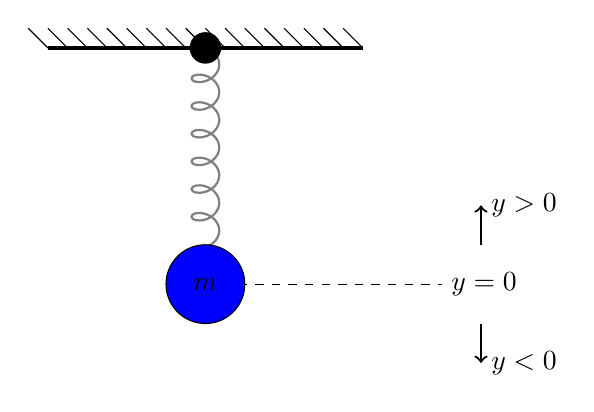
\begin{tikzpicture}
    \draw[ultra thick, black] (-2,0) -- (2,0);
    \foreach \k in {-2,-1.75, -1.5, -1.25, -1, -0.75, -0.5, -0.25,
    0, 0.25, 0.5, 0.75, 1, 1.25, 1.5, 1.75, 2}{
        \draw[black] (\k,0) -- (\k-0.25,0.25);
    }
\draw[thick,gray,decorate,decoration={coil,aspect=0.7,amplitude=5}] (0,0) -- (0,-2.8);
\fill (0,0) circle (.2);
\draw[<-, thick] (3.5,-2) node[anchor=west]{$y>0$} -- (3.5,-2.5);
% \draw[<-, thick] (-1.0,-2) node[anchor=east]{$F_d$} -- (-1.0,-2.5);
% \draw[<-, thick] (-2.0,-2) node[anchor=east]{$F_r$} -- (-2.0,-2.5);
\draw[->, thick] (3.5,-3.5) -- (3.5,-4) node[anchor=west]{$y<0$};
\draw[dashed, black] (0,-3) -- (3,-3) node[anchor=west]{$y=0$};
\draw[fill=blue] (0,-3) circle(0.5cm) node{$m$};
\end{tikzpicture}
 
    \parbox{13 true cm}{\caption{\label{fig:3-10-SpringMass} A mass-spring oscillating system connected to a rigid body above with mass
    $m$.  The coordinate system uses $y=0$ as the rest position of the mass with $y>0$
indicating positions above equilibrium and $y<0$ indicating position below equilibrium.}}
   \end{center}
 
\end{figure}

For an ideal linear spring, Hooke's Law states that the restoring force is proportional to the
displacement of the mass from equilibrium: $F_r = - k y(t)$.  The proportionality constant
$k$ is called the spring constant.  In simple terms, Hooke's Law states that if the
mass-spring system has been stretched a long way from equilibrium then the restoring force
will be large.  If, however, the mass-spring system has been stretched only a short way
from equilibrium then the restoring force will be small.  The negative sign indicates that
the force will pull in the opposite direction of the position and, hence, back toward
equilibrium.  Since force is measured in Newtons, the spring constant $k$ has units of
Newtons per meter.

For an ideal linear spring, the force due to drag will oppose the motion in a manner that
is approximately proportional to the velocity of the mass: $F_d = -b y'(t)$.  That is to
say, if the mass is moving quickly then the force due to drag will be large and if the
mass is moving slowly then the force due to drag will be small.  The damping constant has
units of Newtons per meter per second.

External forces, $f(t)$, are any other forces that act on the system.  Examples of such
forces would be the presence of a magnetic field, the presence of upward or downward air
currents, a periodic forcing term such as pushes or pulls on the mass or spring, etc.  

Using Newton's second law \eqref{eqn:NewtonSecond} we can write the balanced forces as
\begin{flalign}
    ma = F_r + F_d + f(t). \label{eqn:mass-spring-forces}
\end{flalign}
Substituting the restoring force, the damping force, and $a = y''$ into
\eqref{eqn:mass-spring-forces} gives the linear second-order differential equation
\begin{flalign}
    my''(t) = -k y(t) - b y'(t) + f(t).
    \label{eqn:mass-spring}
\end{flalign}
Rearranging \eqref{eqn:mass-spring} algebraically gives the standard form for a linear
second-order non-homogeneous differential equation:
\begin{flalign}
    my'' + by' + ky = f(t).
    \label{eqn:mass-spring2}
\end{flalign}
It should be noted that the forms of $F_r$ and $F_d$ used to build
\eqref{eqn:mass-spring2} are idealizations.  If the spring is stretched {\it too far}, if the
speeds are {\it too high}, or if the materials used are atypical in some way then
different forms of the restoring and damping forces may be necessary.


In this problem we investigate how the mass-spring system \eqref{eqn:mass-spring2} can be
described in terms of potential and kinetic energy.  We begin with a few definitions:
\begin{itemize}
    \item {\bf Kinetic Energy}, the energy of motion, is defined as
        \[ E_{kinetic}(t) = \frac{\text{mass $\times$ velocity$^2$}}{2} = \frac{1}{2} m
            \left[ y'(t)\right]^2. \]
    \item {\bf Potential Energy} in a mass-spring system, also called the {\it
            elastic potential}, is defined as
            \[ E_{potential}(t) = \frac{\text{spring constant $\times$ position$^2$}}{2} =
                \frac{1}{2} k \left[ y(t) \right]^2. \]
    \item The {\bf Total Energy} in a mechanical system is the sum of the
                kinetic energy and the potential energy.
                \[ E_{total}(t) = E_{kinetic}(t) + E_{potential}(t) \]
\end{itemize}
The units of energy are Newton-Meters or Joules.  In terms of a mass-spring system, kinetic energy is the
energy that the mass has due to its motion.  If the mass is at rest then the kinetic
energy is zero.  Also, if the mass has reached a maximum displacement (and is just about
to turn around and move in the opposite direction) the kinetic energy will be zero. The
potential energy in a mass-spring system is the energy that the mass has relative to its
equilibrium position.  If the mass is at equilibrium then it has no potential energy but
if the mass is far from equilibrium it will have a large amount of potential energy.  

\subsection*{Student Tasks:}
The following tasks ask you to explore the mass-spring system by examining the total
energy of the system.  The tasks are necessarily open ended meaning that each group could
(and should) get different answers for each task.  You should use the MATLAB file provided
on the Moodle page for this exploration.  At the end of the explorations you will
write your results in a formal lab report.
\begin{enumerate}
    \item {\bf Make a conjecture}:  In what cases (related to $m$, $b$, $k$, and $f(t)$) do
        you think that the total energy will be constant? Give a few sentences to support
        your claim and then create plots of position, potential energy, kinetic energy,
        and total energy to graphically verify your conjecture. 

    \item {\bf More conjectures}:  In what cases (related to $m$, $b$, $k$, and $f(t)$) do
        you think that the total energy will be decreasing, increasing, or
        oscillating in a mass-spring system? Give a few sentences to support your claims.



    \item {\bf Exploration:} Fully explore how the energy behaves in the mass-spring
        system.  To make your exploration somewhat easier let's assume the following:
        \[ \text{mass}=m=1\text{kg}, \quad \text{initial position }=y(0) = 0\text{m}, \quad \text{initial
        velocity}=y'(0)=1\text{m/sec}. \]
        This way you only have the damping constant $b$, the restoring constant $k$, and
        the forcing function $f(t)$ to experiment with.  The given initial conditions will
        start the mass at equilibrium and given it an initial upward velocity.

Use the background information presented earlier in this document to conjecture and test
combinations of $b$, $k$, and $f(t)$ that result in the following situations.  You must
find the situations listed, and the last item in the following list gives you a chance to
look for situations that are not listed.   
\begin{enumerate}
    \item Find a combination of parameters where the total energy drops slowly to zero.
    \item Find a combination of parameters where the total energy drops very quickly to
        zero.
    \item Find a combination of parameters where  the total energy oscillates but never
        reaches zero and does not increase for all time.
    \item Find a combination of parameters where the total energy increases for all time.
    \item Find a combination of parameters where the total energy changes initially but
        eventually finds a nonzero equilibrium.
    \item Find a combination of parameters where the system exhibits resonance (where the
        unforced frequency matches the frequency of the forcing term).
    \item Find a combination of parameters where the total energy oscillates with two
        frequencies: a slow frequency and a faster frequency (hint: get the resonant
        system first and then change the frequency of the forcing term).
    \item Now go find several other combinations of parameters that give behaviors
        different than the ones listed above.
\end{enumerate}

\item {\bf Summary:} Summarize all of your findings into a well-formated lab report clearly showing the
    mathematical and graphical representations all of the cases used in your
    experimentations.  Your initial conjectures (from problems 1 and 2) may have been
    incorrect so take this chance to clarify what you've found.  Your summary must include
    general descriptions of the following four general scenarios. 
    \begin{enumerate}
        \item The total energy remains constant.
        \item The total energy drops to zero.
        \item The total energy increases without bound.
        \item The total energy oscillates.
    \end{enumerate}

\end{enumerate}



\section{Modeling Explorations with $2^{nd}$ Oder Differential Equations}
\begin{problem}
    A large water tower holds 3 million gallons of water, which has a mass of about 11
    million kilograms.  When the wind blows, this causes the steel structure to sway back
    and forth due to the force.  An engineer studying the tower observes that a steady
    wind at a speed of 35 mph exerts a force of 1.45 million Newtons on the tower, causing
    it to lean 0.27 meters away from equilibrium.  The engineer begins by assuming that
    the restoring force is proportional to the displacement $F = - k x$, so that the motion
    of the system can be modeled by the differential equation $m a = -k x$.  Here $m$ is the
    mass of the tower, $a$ is the tower's acceleration, $k$ is the spring constant, and $x$ is
    the displacement of the tower away from its equilibrium position.
    \begin{enumerate}
        \item[(a)] What is the spring constant of the steel structure?  (Be sure to
            use the right units!)
        \item[(b)] What is the angular frequency $\omega$ at which the tower will tend to oscillate?
            (Note that angular frequency is measured in radians per second.)
        \item[(c)] Write down the general solution to the differential equation.  (This is
            the version with the two arbitrary constants that we will have to figure out
            from the initial conditions.)
        \item[(d)] Suppose that the tower is sitting comfortably in equilibrium when a sudden
            brief gust of wind gives the tower a velocity of $+0.24$ meters per second.
            What function will describe how the position of the tower changes after this?
        \item[(e)] Make a plot of this function.
        \item[(f)] What is the maximum displacement away from equilibrium that the water
            tower goes? (Use your graph as an aid, but use your function from (d) to get
            the exact value.)
        \item[(g)] Reading from your graph, what is the period of oscillation?  That is, how
            much time does it take the tower to go through one complete back-and-forth
            cycle?
        \item[(h)] How would your plot be different if there had been a stronger gust of
            wind?  What would be the same and what would be different?
        \item[(i)] What function describes the velocity of the tower?
        \item[(j)] Make a plot of velocity versus
            time in.
        \item[(k)] What is the maximum speed that the water tower attains?  (Speed is the
            absolute value of velocity.) Again, use both your graph and your velocity
            function.
        \item[(l)] Where is the water tower when it is moving the fastest?
        \item[(m)] Compare your plot of position versus time with your plot of velocity
            versus time.  You will find that first the velocity reaches a positive peak,
            then position follows, then velocity reaches a negative peak, then position
            follows, etc.  Why is this?  Explain in terms of the motion of the physical
            object.
        \item[(n)] What function describes the acceleration of the tower?
        \item[(o)] Make a plot of acceleration versus
            time.
        \item[(p)] What is the greatest acceleration experienced by the tower?
        \item[(q)] Where is the tower when it is accelerating the most?
        \item[(r)] Another way to analyze motion is to create a phase plot, which puts
            velocity on the y-axis and position on the x-axis.  Create a plot like this.
        \item[(s)] This is a strange looking plot!  What point on this plot represents our
            initial condition?  
        \item[(t)] What is going on when the tower is at a point on the far left side of this
            curve?
        \item[(u)] Would the motion of the water tower cause this curve to be traversed in a
            clockwise or a counterclockwise direction?  Explain your thinking.
        \item[(v)] Suppose that a month later, the tower is holding 21.5 million kilograms of
            water, when it experiences a gust of wind that again gives it a speed of 0.24
            m/s.  What function will describe the displacement of the tower?
        \item[(w)] Make a plot of the resulting position as a function of time.
        \item[(x)] Now what is the period of oscillation?  (Estimate from graph and confirm
            with position function.)
        \item[(y)] The steel framework will experience catastrophic structural failure if it
            sways more than 1.2 meters.  What is the maximum speed that a gust of wind can
            give the tower while it's holding 21.5 million kg of water before this causes
            unpleasant results?
        \item[(z)] Another engineer studies a similar tower in the neighboring town, finding that
            while this contains only 9.5 million kilograms of water, it tends to sway back
            and forth with an angular frequency of  = 0.55 rad/s.  What must be the spring
            constant of the structure holding up this water tower?
    \end{enumerate}
\end{problem}


\begin{problem}
    If we construct an electrical circuit with a capacitor and an inductor in series we
    find that the amount of charge on the capacitor $Q(t)$ (with charge measured in
    Coulombs) can be modeled by the following differential equation:
    \[ L \frac{d^2 Q}{dt^2} + \frac{Q}{C} = 0, \]
    where C is the capacitance of the capacitor as measured in Farads, and $L$ is the
    inductance of the inductor as measured in Henrys, and the second derivative has units
    of Coulombs/second$^2$.
    \begin{enumerate}
        \item[(a)] If we have $C=2\times 10^{-6}$F and $L=2$ Henrys, what is the general solution to this
            differential equation? 
        \item[(b)] Your answer to the first question should include the constant ``500.''  What
            units does this number have?  This is called the natural frequency of the
            circuit.
        \item[(c)] What is the period of these oscillations?
        \item[(d)] Suppose we begin with 8 nanocoulombs of charge on the capacitor and no
            current flowing through the circuit ($Q'(t)=0$).  What solution function
            corresponds to this set of initial conditions?
        \item[(e)] Create a graph showing how the charge on the capacitor varies over time.
            Your graph should begin at $t = 0$ and should show only a few periods of
            oscillation.
        \item[(f)] How much charge is on the capacitor at $t = 10$ milliseconds?
        \item[(g)] New scenario:  Suppose we begin with no charge on the capacitor, but
            charge flowing through the circuit at a rate of 25 millicoulombs per second.
            (This is the same as 25 milliamps.)  What solution function corresponds to
            this set of initial conditions?
        \item[(h)] In this scenario:  What is the maximum amount of charge on the capacitor?
            Give your answer in microcoulombs.
        \item[(i)] Create a graph showing how the charge on the capacitor varies over time.
            Your graph should begin at $t = 0$ and should show only a few periods of
            oscillation.
        \item[(j)] Now, suppose we begin with 10 microcoulombs of charge on the capacitor and
            10 milliamps of charge flowing through the circuit.  What solution function
            corresponds to this set of initial conditions?

        \item[(k)] What is the maximum amount of charge on the capacitor?
        \item[(l)] If we add an antenna to this circuit, then the voltage from the antenna
            $V(t)$ will be added to the differential equation like this:
            \[ L \frac{d^2 Q}{dt^2} + \frac{Q}{C} = V(t). \]

            Find a function that will serve as a particular solution to this differential
            equation with an antenna signal of   
        \item[(m)] What is the maximum amount of charge on the capacitor produced by this
            particular solution?
        \item[(n)] What is the period of oscillation found in your particular solution?
            State your answer in milliseconds.
        \item[(o)] Create a graph showing how the charge on the capacitor varies over time.
            Your graph should begin at $t = 0$ and should show only a few periods of
            oscillation.
        \item[(p)] A radio uses a circuit like this in order to amplify one frequency, the
            frequency of the station that you want to listen to, while ignoring the
            frequencies of the other stations.  The circuit has a variable capacitor and
            when the natural frequency of the circuit matches the antenna frequency that
            you want amplified, then the circuit produces a behavior called “resonance.”
            If the inductor remains constant at $L=2$  Henrys, then what capacitance C do we
            need in order for the circuit to have resonance with an antenna signal at a
            frequency of 600 radians per second?
    \end{enumerate}
\end{problem}
